\section{Results} \label{sec:cba_results}
This section discusses running the GTT aircraft through the modified flight certification maneuver.
There are two overarching goals of this work: first, to provide a framework that brings flight testing earlier in the aircraft design process, and second, to create the most accurate flight simulation results while minimizing the cost of the underlying analyses. 
To this end, this section first focuses on comparing simulations run using purely high-fidelity experimental data to those run using low-fidelity and multi-fidelity data that would be available early in the design process.
Then the cost-reduction aspect is explored by harnessing the benefits of multi-fidelity databases that use small subsets of the high-fidelity data. 
For all the results in this section, simulations are conducted with the right engine inoperative, and all modifications discussed in Section \ref{subsec:sim_mods} are applied.

\subsection{Simulations using Single- vs. Multi-Fidelity Databases} \label{subsec:sf_vs_mf_cba}

In the nascent stages of aircraft design, engineers use low-fidelity methods, such as AVL simulations, to perform rapid analyses that can span vast regions of the design domain quickly. 
These have higher uncertainties in their performance predictions due to simplifications made in modeling the flow physics in favor of speed of analysis.
As parts of the aircraft design get fixed, engineers employ higher-fidelity methods such as RANS CFD simulations to perform design optimizations.
These are computationally more expensive than AVL simulations and provide a more accurate representation of the aircraft's potential performance. 
Once designs get finalized, manufactured prototypes are experimentally tested in wind tunnels. 
These provide high-fidelity data that can recreate the expected flight conditions and have correspondingly low uncertainties associated with their performance predictions.
After finalizing all design decisions and manufacturing a full-scale prototype, real-world flight testing certifies the aircraft's airworthiness.

Mimicking this sequence of design analyses, single- and multi-fidelity databases that use, in order, low-fidelity (AVL), low- + medium-fidelity (AVL + SU2), and low- + medium- + high-fidelity (AVL + SU2 + WT) data are created. 
Section \ref{sec:data_gen} presented an example of this build-up.
Flight simulations using these lower- and multi-fidelity databases bring aspects of the real-world flight testing procedure into the virtual environment where engineers perform the early design analyses.
To assess the quality of the results, they are compared to flight simulations carried out using high-fidelity databases created using only experimentally obtained wind tunnel data. 
It is important to note that while wind tunnel data has its own set of models that introduce errors compared to flight tests, it is the highest-fidelity data available and is considered the truth function being emulated. 

It is important to remember that limited aerodynamic data is available from SU2. 
This limitation means that the two-fidelity results only use SU2 data for the force and moment coefficients in the aerodynamics database.
The controls databases for the two-fidelity results are only single-fidelity and are identical to the controls databases used for the AVL-only results. 
Consequently, the three-fidelity database is only three-fidelity for the force and moment coefficients; the rest are two-fidelity.
The overall results are still referred to as two-fidelity when using AVL+SU2 data and three-fidelity when using AVL+SU2+WT data to avoid verbose explanations.

\begin{figure}
    \centering
    \begin{subfigure}[CDF for the trim $\alpha$]{
        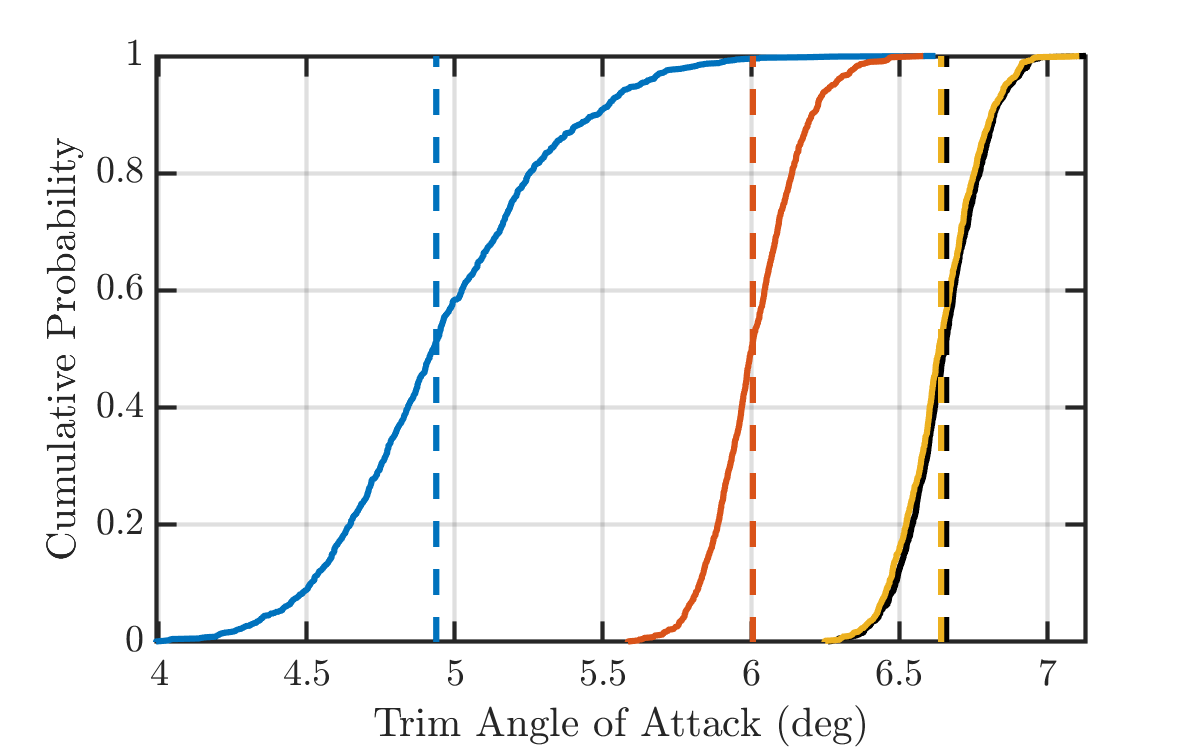
\includegraphics[trim=0 0 0 0, clip, width=.48\textwidth]{code/image_gen/cba/Stanford_CFR25_147d_2_R2/images/trim_aoa_sf_vs_mf.png} 
        \label{subfig:sf_vs_mf_trim_cdf}
    } 
    \end{subfigure}
    \hfill
    \begin{subfigure}[CDF for the pitch metric]{
        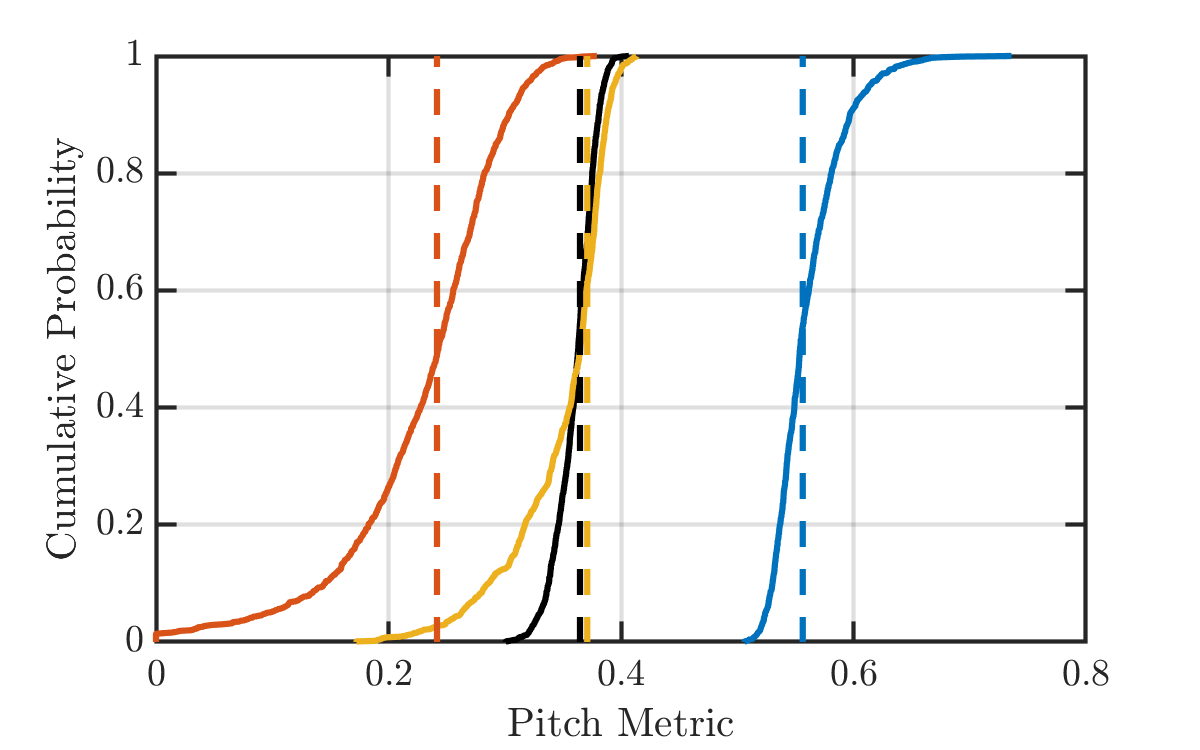
\includegraphics[trim=0 0 0 0, clip, width=.48\textwidth]{code/image_gen/cba/Stanford_CFR25_147d_2_R2/images/reo_pitch_sf_vs_mf.png} 
        \label{subfig:sf_vs_mf_pitch_cdf}
    } 
    \end{subfigure}
    \hfill
    \begin{subfigure}[CDF for the roll metric]{
        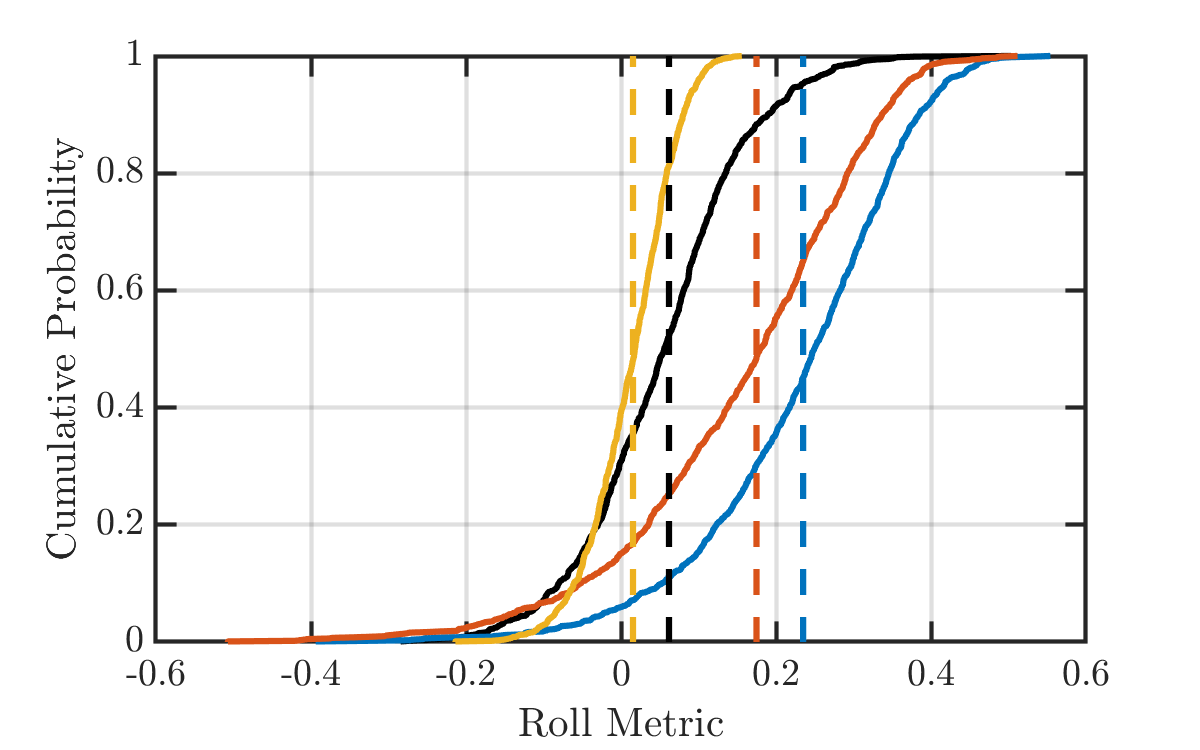
\includegraphics[trim=0 0 0 0, clip, width=.48\textwidth]{code/image_gen/cba/Stanford_CFR25_147d_2_R2/images/reo_roll_sf_vs_mf.png} 
        \label{subfig:sf_vs_mf_roll_cdf}
    } 
    \end{subfigure}
    \hfill
    \begin{subfigure}[CDF for the yaw metric]{
        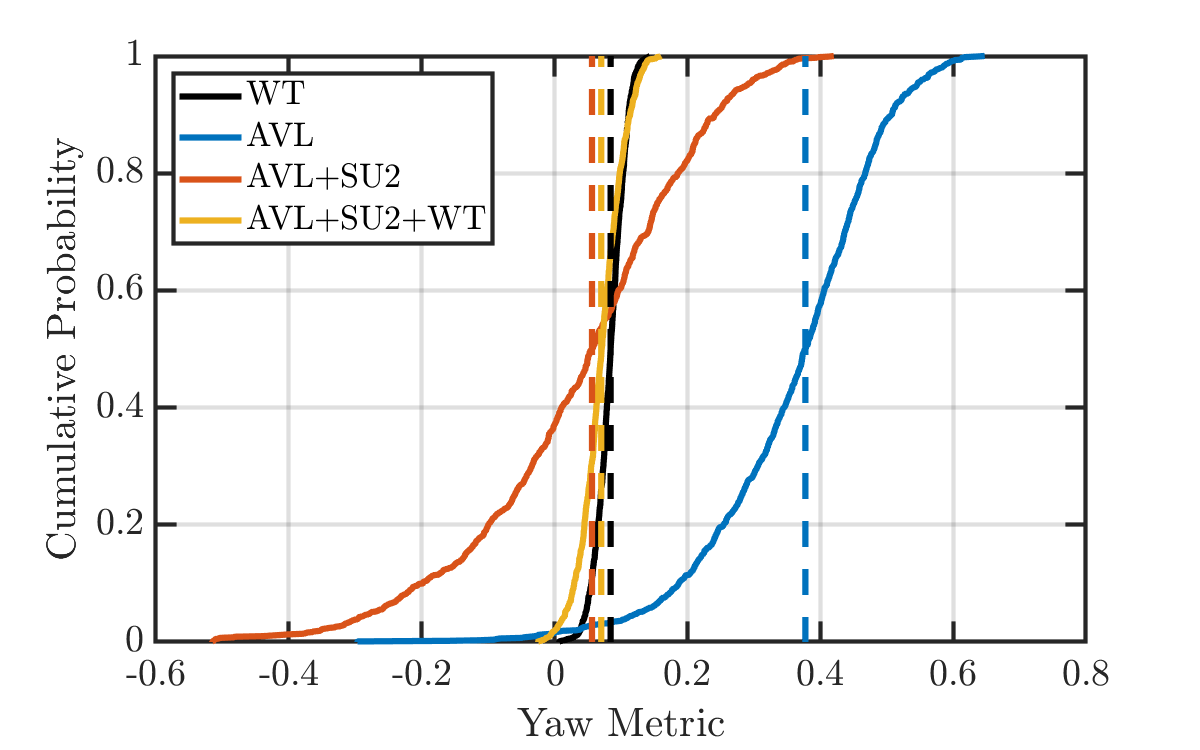
\includegraphics[trim=0 0 0 0, clip, width=.48\textwidth]{code/image_gen/cba/Stanford_CFR25_147d_2_R2/images/reo_yaw_sf_vs_mf.png} 
        \label{subfig:sf_vs_mf_yaw_cdf}
    } 
    \end{subfigure}
    \caption{Comparing flight simulations of the certification maneuver when different combinations of low-, multi-, and high-fidelity databases are used. CDF plots for the trim angle of attack and the success metrics are shown. \label{fig:sf_vs_mf_metric_cdfs}}
\end{figure}

With the details of the simulation procedure explained in Section \ref{sec:sim_procedure}, the results here will be presented primarily through the CDF plots of the success metrics resulting from the Monte Carlo analysis defined in \ref{subsec:mc_analysis}.

Figure \ref{fig:sf_vs_mf_metric_cdfs} presents the results of the flight simulations when lower fidelity databases are used.
Early in the conceptual design stages, the aircraft performance would be determined using low-fidelity analyses, and the flight simulations would yield the results represented by the blue line. 
The significant uncertainties attributed to the AVL analyses yield a large variance in the metrics, indicated by the wide range of values that the CDF spans for every metric.
AVL over-predicts the effectiveness of all control surfaces with the CDF for each metric lying to the right of the other results, indicating lower control surface saturation during the simulations. 

Progressing with the aircraft design, we add RANS CFD data to the GP models.
The red line represents the results of flight simulations using AVL+SU2 data. 
The effect of having the more accurate aerodynamic force and moment coefficients is evident, especially in calculating the trim angle of attack shown in Figure \ref{subfig:sf_vs_mf_trim_cdf}.
Since no additional data improves the controls databases, the simulations preserve the significant variance in success metrics seen in the AVL results. 
Nevertheless, the additional accuracy in the baseline aerodynamics shifts all of the two-fidelity results closer towards the three-fidelity and high-fidelity results.

With the addition of the wind tunnel data to the multi-fidelity fit (yellow line), the flight simulation results should be very close, if not identical, to those using the single-, high-fidelity data (black line). 
The trim angles of attack, pitch metrics, and yaw metrics line up identically. 
However, there is a notable difference in the roll metric results. 
Not only is the mean value for the three-fidelity database (dashed yellow line) lower than that for the single-, high-fidelity database, but the variance in the roll metric is also lower. 
The reason for this difference was hinted at in Section \ref{sec:gtt_dbs} when comparing the single- and multi-fidelity databases for $C_{l{\delta_a}}$. 
This is highlighted in Figure \ref{fig:sf_vs_mf_crmail} when plotting samples of the databases as a function of $\delta_a$ when $\alpha=8^\circ$ and $\beta = 4^\circ$.

\begin{figure}
    \centering
    \begin{subfigure}[Single-, high-fidelity database]{
        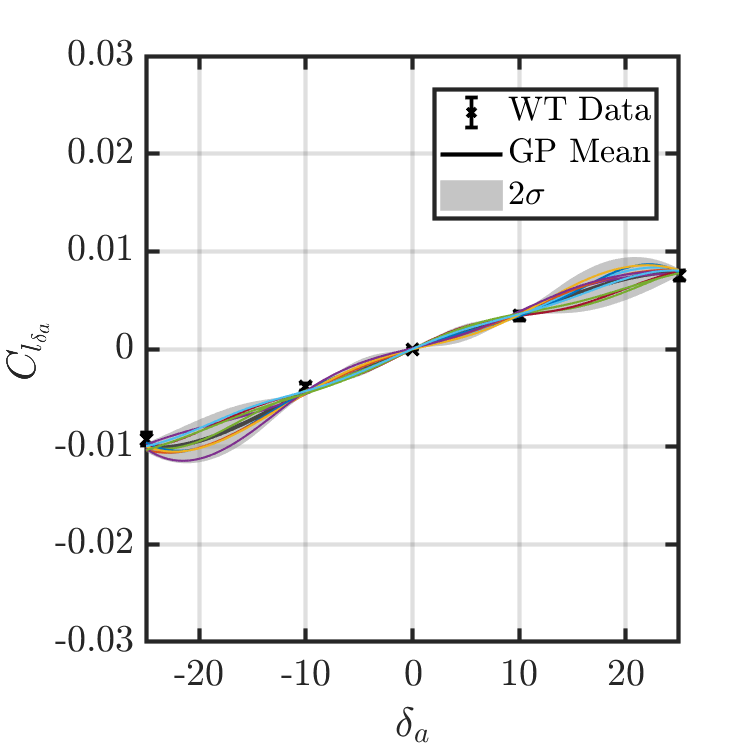
\includegraphics[trim=0 0 0 0, clip, width=.48\textwidth]{code/image_gen/gmatt/1f/wt_old/images/gps/CRMAIL_alpha=8_beta=4+samps.png} 
        \label{subfig:sf_crmail}
    } 
    \end{subfigure}
    \hfill
    \begin{subfigure}[Multi-fidelity database]{
        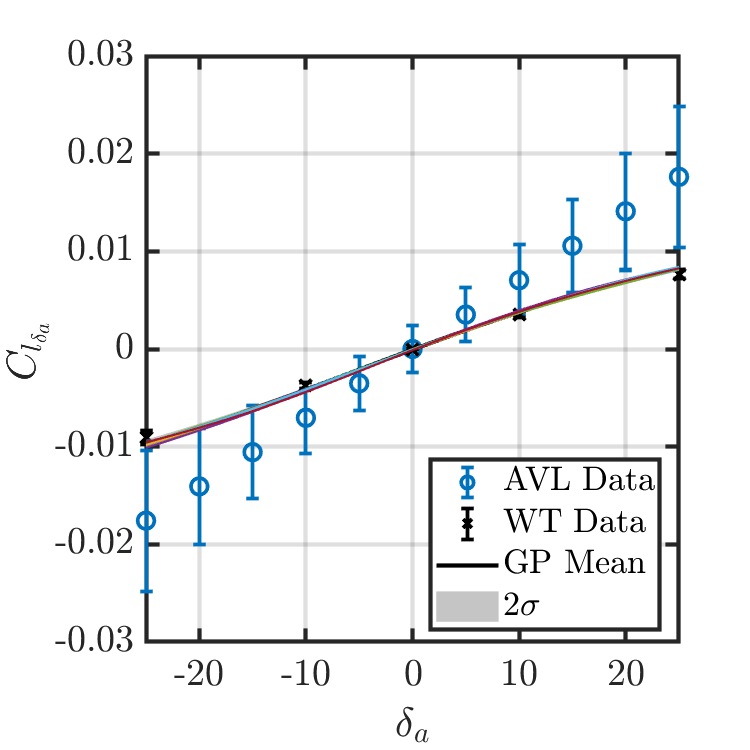
\includegraphics[trim=0 0 0 0, clip, width=.48\textwidth]{code/image_gen/gmatt/3f/images/gps/CRMAIL_alpha=8_beta=4+samps.png} 
        \label{subfig:mf_crmail}
    } 
    \end{subfigure}
    \caption{Comparing $C_{l_{\delta_a}}$ as a function of $\delta_a$ when single-, high-fidelity data is used vs. when multi-fidelity data is used. The individual colored lines represent samples of the database. \label{fig:sf_vs_mf_crmail}}
\end{figure}

When using purely wind tunnel data to create the databases, Figure \ref{subfig:sf_crmail}, the sparsity of data points in the aileron deflection dimension results in the ballooning GP error estimate between available data points (the black squares).
The database samples, $10$ of which are shown by the individual colored lines,  respect the error estimate from the GP and have correspondingly higher variability between those data points.
When supplemented with lower-fidelity AVL data (blue circles), the multi-fidelity GP can use the trends learned from the lower fidelity to reduce the uncertainty between the same set of wind tunnel data points. 
As a result, the error estimate from the GP is lower and is barely discernible at the scale of the figure. 
The samples show significantly less variation from the mean database and are almost all coincident in this case. 
Consequently, there is a lower variance in the roll metric as indicated by the CDF plot for the three-fidelity case in Figure \ref{subfig:sf_vs_mf_roll_cdf}.

This observation brings to question the assumption of using the single-, high-fidelity database results as the truth function being emulated. 
The increased error estimates between data points do not indicate a failure of the GP model in learning the correct trends; instead, it suggests that data sampling is sparse and reducing the uncertainty in the model requires more data.
The advantage of using multi-fidelity data is clear. 
The uncertainty in the model can be reduced without any new, expensive, high-fidelity function evaluations.

\begin{table}
\centering
    \renewcommand{\arraystretch}{1.2}
    \captionsetup{justification=centering}
    \caption{Mean, variance, and failure rate for the flight certification maneuver when using different aircraft databases.} 
    \begin{tabular}{|c|c|c|c|c|c|c|c|c|c|}
    \hline
        Case & \multicolumn{3}{c|}{Pitch Metric} & \multicolumn{3}{c|}{Roll Metric} & \multicolumn{3}{c|}{Yaw Metric} \\ \hline
         & $\mu$ & $\sigma^2$ & Failure & $\mu$ & $\sigma^2$ & Failure & $\mu$ & $\sigma^2$ & Failure \\ \hline
        AVL & 0.56 & 8.21e-04 & 0.0\% & 0.23 & 1.83e-02 & 6.0\% & 0.36 & 1.70e-02 & 1.6\% \\ \hline
        AVL+SU2 & 0.23 & 4.59e-03 & 0.0\% & 0.16 & 2.45e-02 & 15.1\% & 0.04 & 2.87e-02 & 37.1\% \\ \hline
        AVL+SU2+WT & 0.35 & 1.76e-03 & 0.0\% & 0.01 & 3.04e-03 & 39.2\% & 0.08 & 4.73e-04 & 0.0\% \\ \hline
        WT & 0.36 & 2.87e-04 & 0.0\% & 0.05 & 1.13e-02 & 30.8\% & 0.08 & 4.74e-04 & 0.0\% \\ \hline
    \end{tabular}
    \label{tab:sf_vs_mf_perf_stats}
\end{table}

Table \ref{tab:sf_vs_mf_perf_stats} presents the relevant statistics for the same set of simulations represented in Figure \ref{fig:sf_vs_mf_metric_cdfs}.
$\mu$ and $\sigma^2$ represent the sample mean and variance of the metrics.
The trends noticed visually in the CDF plots are confirmed by the numbers in the table. 
Looking at the simulation results from the perspective of flight certification, the main QoI is the failure rate for the air-worthiness maneuver. 
The failure rate is defined as the percentage of cases for which the metric $\rho_* < 0$.
The modifications in the maneuver simulations listed in Section \ref{subsec:sim_mods} result in higher failure rates compared to those shown in Section \ref{sec:sim_procedure}.
None of the databases have any failures in the pitch metric. 
AVL overestimates the control effectiveness of all the control surfaces as mentioned earlier.
This factor underestimates the roll metric failure rate when using only AVL data for the controls databases. 
The overestimated control effectiveness is also seen in the yaw metric, but the high uncertainty in the databases leads to more failures. 

These trends urge caution when relying on purely low-fidelity analyses to make control-sizing decisions early in the design process.
The overestimation of control-effectiveness by these low-fidelity methods needs addressing to correlate with high-fidelity simulations better. 
It does not mean that performing early flight simulations are not helpful, just that necessary corrections would need to be derived and applied to make meaningful inferences from the data. 
Perhaps constraints on acceptable performance at early design stages would need to be different from those used for later stages. 
For example, acceptable performance in the conceptual design stage could require successful flight simulations with half the full range of motion for the control surfaces planned for the actual design.
This suggestion is already employed here as the simulation modifications made in Section \ref{subsec:sim_mods} reduced the allowable range of motion for the ailerons and the rudder. 

Aircraft manufacturers often use such rules-of-thumb and factors of safety.
Historical data using previously certified aircraft and all the analyses performed during their design process can be used to create these corrections. 
Since most of the required data is proprietary, deriving these corrections is outside of the scope of this work. 

\subsection{Simulations using Reduced Data}

A significant advantage of using multi-fidelity data to create surrogate models is that the underlying function in question can be approximated better with fewer high-fidelity function evaluations.
This has been published on extensively, \cite{kennedy_predicting_2000,gratiet_multi-fidelity_nodate,perdikaris_multi-fidelity_2015, ghoreishi_gaussian_2018}, to name a few. 
Earlier in this work, Section \ref{sec:mf_modeling} shows this property for analytic functions and Section \ref{sec:mf_gp_nasa_crm} shows it for single- and multi-dimensional aerodynamic databases.
With the NASA CRM databases, the advantage is evident in both cases, when high-fidelity evaluations are uniformly spaced and when localized to areas where the low-fidelity data is inadequate. 
This section explores the effect of the flight simulation procedure on this advantage.

To explore this, we create three new sets of databases for the GTT:
\begin{enumerate}
    \item WT-Coarse: Single-fidelity GP only using a sparse subset of the available wind tunnel data.
    \item 3F-Coarse: Multi-fidelity GP using all the AVL and SU2 data, but uses a sparse subset of the wind tunnel data (same subset at WT-Coarse).
    \item 3F-Local: Multi-fidelity GP  using all the AVL and SU2 data, and supplementing it with a subset of the wind tunnel data localized to high values of $\alpha, \beta,$ and $\delta_*$.
\end{enumerate}

The sparse subset of the wind tunnel data uses data for every $4^\circ$ change in angle of attack.
This coarsening equates to using $\approx20\%$ of all the experimental data available for the aerodynamics database, and $\approx40\%$ of the experimental data available for the controls database. 
This level of data reduction would equate to significant cost savings in experimental analyses while allowing an even spread of data over the domain of interest. 
The WT-Coarse and the 3F-Coarse databases use the same sparse subset of wind tunnel data.

With the 3F-Local database, the idea is to localize the high-fidelity evaluations to certain domain regions.
It simulates a situation where if high-quality low-fidelity data is available in certain parts of the domain, high-fidelity evaluations in those areas would be an unnecessary expense. 
Instead, engineers can focus the limited resources on areas where the low-fidelity data is inadequate or has very high uncertainty associated with it. 
Both AVL and RANS CFD simulations are inaccurate when there is significant flow separation over the aircraft. 
This occurs at high values of $\alpha, \beta,$ and $\delta_*$.
To this end, for the 3F-Local database, high-fidelity data is limited to areas of the domain where $\alpha > 10^\circ, \beta > 10^\circ,$ and $\delta_* > 15^\circ$.

Continuing with the use of CDF plots, Figure \ref{fig:red_data_metric_cdfs} shows the results of using the different subsets of the wind tunnel data.
Statistics of the metric distrubutions are shown in Table \ref{tab:red_data_perf_stats}.
The different databases are compared to the same single-, high-fidelity database used in the previous section.

An overarching trend across the four plots is that the variance in the metrics increases when using a subset of the high-fidelity data. 
Having fewer data points increases the uncertainty in the GP predictions.
It leads to more significant variability in the database samples and, consequently, greater variance in the output metrics from the flight simulations. 

\begin{figure}
    \centering
    \begin{subfigure}[CDF for the trim $\alpha$]{
        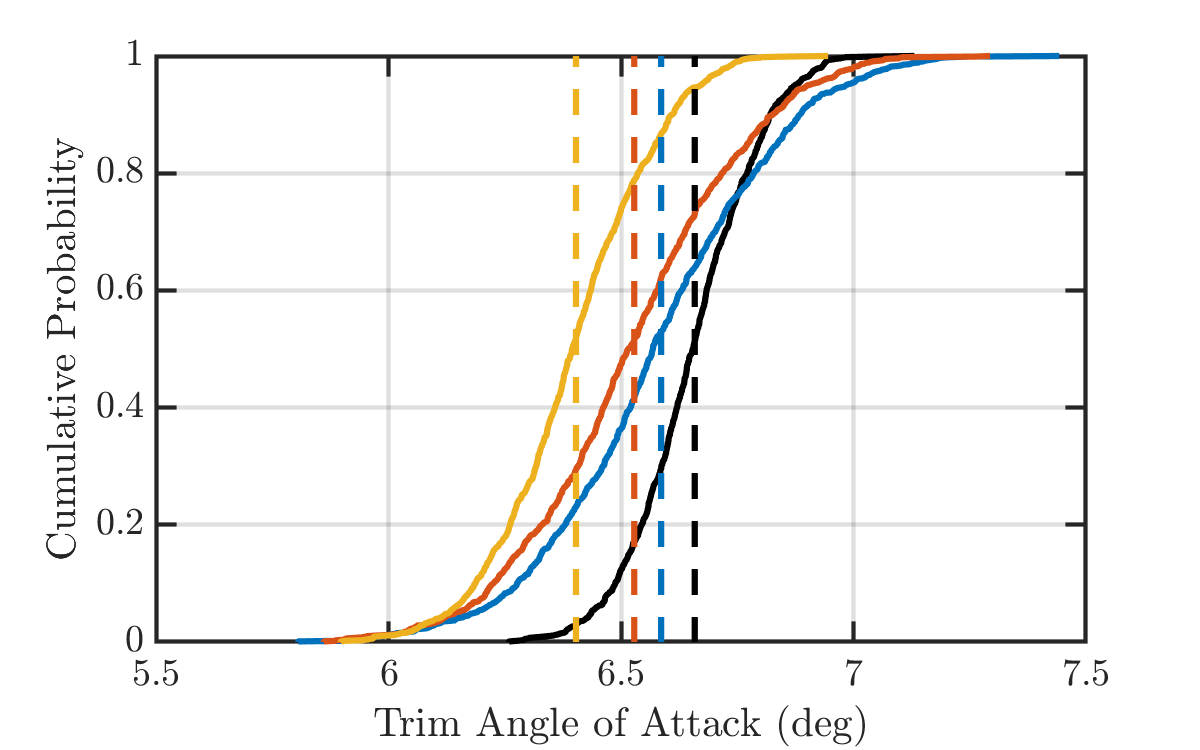
\includegraphics[trim=0 0 0 0, clip, width=.48\textwidth]{code/image_gen/cba/Stanford_CFR25_147d_2_R2/images/trim_aoa_reduced_data.png} 
        \label{subfig:red_data_trim_cdf}
    } 
    \end{subfigure}
    \hfill
    \begin{subfigure}[CDF for the pitch metric]{
        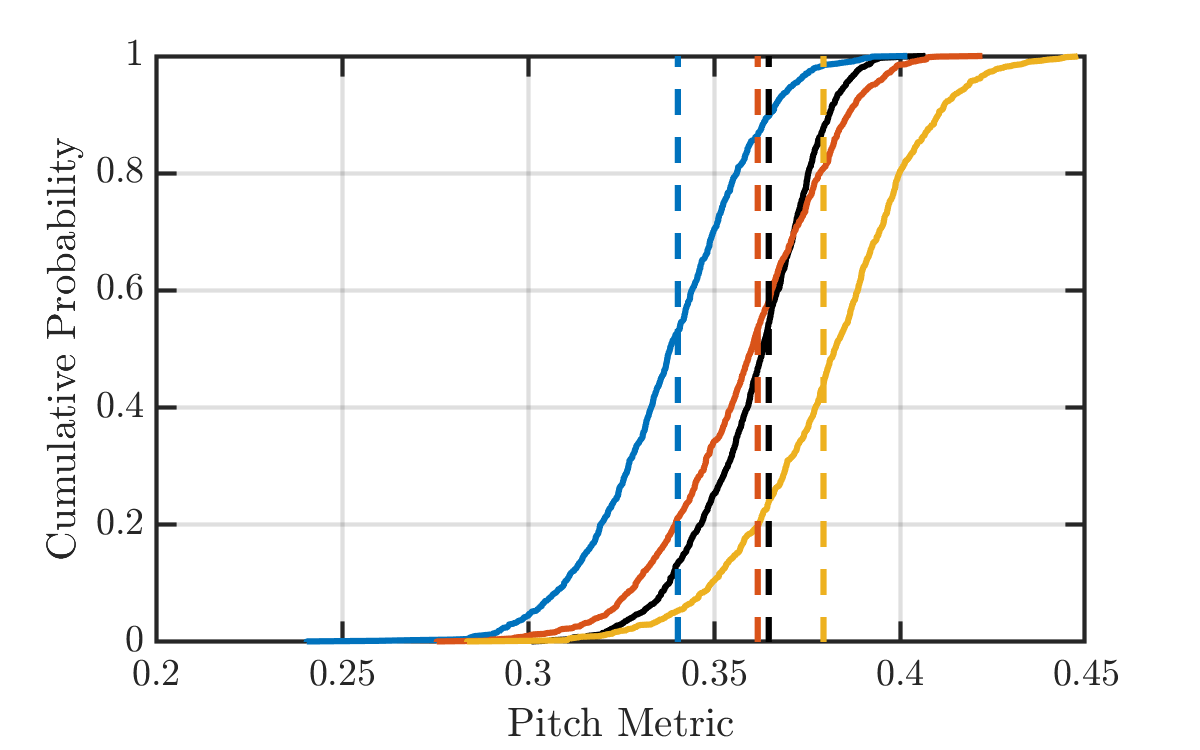
\includegraphics[trim=0 0 0 0, clip, width=.48\textwidth]{code/image_gen/cba/Stanford_CFR25_147d_2_R2/images/reo_pitch_reduced_data.png} 
        \label{subfig:red_data_pitch_cdf}
    } 
    \end{subfigure}
    \hfill
    \begin{subfigure}[CDF for the roll metric]{
        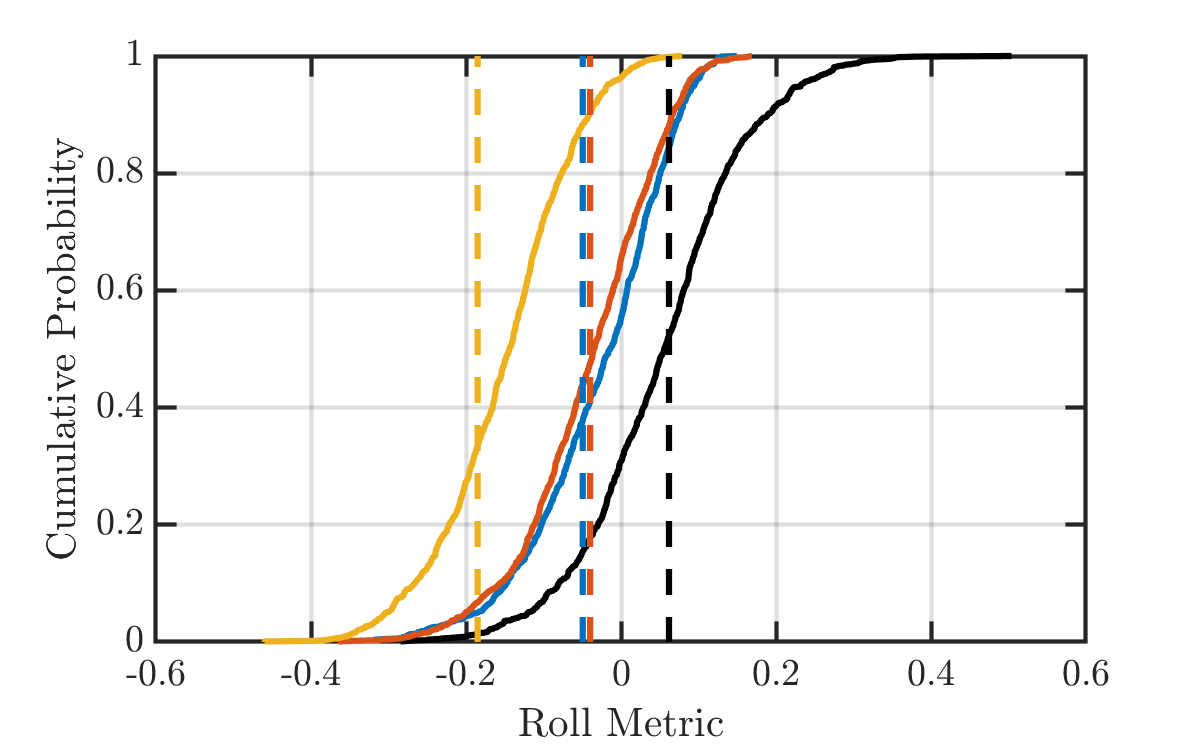
\includegraphics[trim=0 0 0 0, clip, width=.48\textwidth]{code/image_gen/cba/Stanford_CFR25_147d_2_R2/images/reo_roll_reduced_data.png} 
        \label{subfig:red_data_roll_cdf}
    } 
    \end{subfigure}
    \hfill
    \begin{subfigure}[CDF for the yaw metric]{
        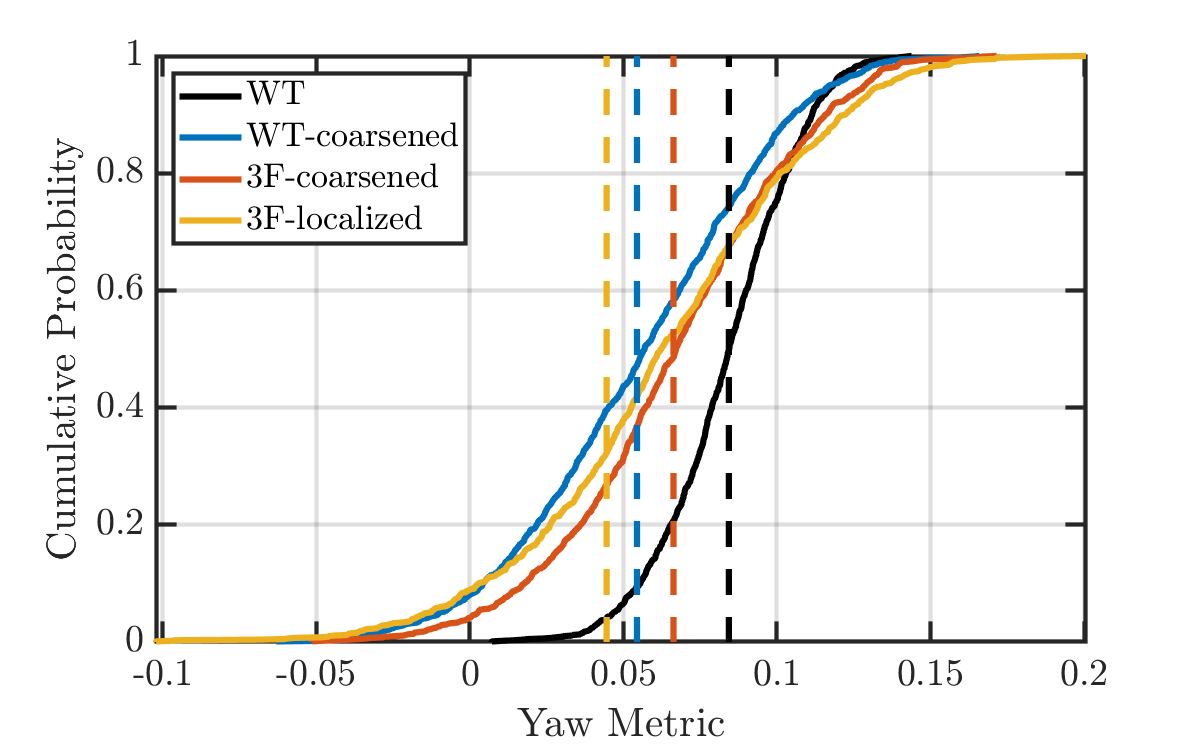
\includegraphics[trim=0 0 0 0, clip, width=.48\textwidth]{code/image_gen/cba/Stanford_CFR25_147d_2_R2/images/reo_yaw_reduced_data.png} 
        \label{subfig:red_data_yaw_cdf}
    } 
    \end{subfigure}
    \caption{Comparing flight simulations of the certification maneuver when subsets of the high-fidelity experimental data is used. CDF plots for the trim angle of attack and the success metrics are shown. \label{fig:red_data_metric_cdfs}}
\end{figure}

\begin{table}
\centering
    \renewcommand{\arraystretch}{1.2}
    \captionsetup{justification=centering}
    \caption{Mean, variance, and failure rate for the flight certification maneuver when using different subsets of high-fidelity data.} 
    \begin{tabular}{|c|c|c|c|c|c|c|c|c|c|}
    \hline
        Case & \multicolumn{3}{c|}{Pitch Metric} & \multicolumn{3}{c|}{Roll Metric} & \multicolumn{3}{c|}{Yaw Metric} \\ \hline
         & $\mu$ & $\sigma^2$ & Failure & $\mu$ & $\sigma^2$ & Failure & $\mu$ & $\sigma^2$ & Failure \\ \hline
        WT & 0.36 & 2.87e-04 & 0.0\% & 0.05 & 1.13e-02 & 30.8\% & 0.08 & 4.74e-04 & 0.0\% \\ \hline
        WT-Coarse & 0.34 & 4.60e-04 & 0.0\% & -0.03 & 7.87e-03 & 55.2\% & 0.06 & 1.54e-03 & 8.0\% \\ \hline
        3F-Coarse & 0.36 & 4.97e-04 & 0.0\% & -0.04 & 7.68e-03 & 65.3\% & 0.07 & 1.41e-03 & 4.2\% \\ \hline
        3F-Local & 0.38 & 5.81e-04 & 0.0\% & -0.15 & 7.38e-03 & 96.4\% & 0.06 & 2.04e-03 & 9.0\% \\ \hline
        
    \end{tabular}
    \label{tab:red_data_perf_stats}
\end{table}

Direct comparison between the WT-Coarse (blue) and the 3F-Coarse data (red) provides an insight into the usefulness of the lower-fidelity data in improving the overall GP mean and uncertainty estimates. 
The most significant difference between the two is for the pitch metric in Figure \ref{subfig:red_data_pitch_cdf}.
The 3F-Coarse database results for the pitch metric are nearly identical to those from the WT database that uses all the wind tunnel data. 
While the WT-Coarse does marginally better at predicting the trim angle of attack (Figure \ref{subfig:red_data_trim_cdf}), 3F-Coarse does marginally better for the roll and yaw metrics (Figures \ref{subfig:red_data_roll_cdf} and \ref{subfig:red_data_yaw_cdf}).

This observation yields that the multi-fidelity fit can perform as well as, if not better than, the single-fidelity fit when there is only sparse high-fidelity data available. 
It is worth reiterating that while we compare results to the single-fidelity WT database, it is not necessarily the best approximation of the actual flight performance.
As seen in the previous section, the uncertainties in the GP model for the WT case can corrupt the expected performance metrics. 
However, in the absence of higher fidelity data than wind tunnel experiments, the wind tunnel data is the primary benchmark. 

The 3F-Local case presents a notable deficiency in the results. 
The addition of localized wind tunnel data improves overall predictions compared to the two-fidelity case shown in the previous section, but it inferior when compared to the other three-fidelity results. 
It cannot get close to the mean metric estimates, nor does it provide a significant reduction in the variance of the performance metrics. 
This deficiency is due to the difference in the low-fidelity and high-fidelity data in areas the high-fidelity data is ignored. 
In these areas, the low-fidelity approximations should capture some of the relevant physics and have correspondingly low uncertainties. 
In reality, RANS CFD simulations only provide some high-quality aerodynamic force and moment coefficient data, while all of the controls databases are built on purely AVL data. 
The high uncertainty and the inadequacy of the AVL data require more than just localized high-fidelity evaluations to improve predictions. 

The data reduction techniques used here are rudimentary. 
Adaptive sampling methodologies leverage the error estimates from the GP models to introduce high-fidelity data at specific locations to minimize the overall uncertainty in the model. 
Simple techniques, such as using high-fidelity data in areas with the highest uncertainty as predicted by the GP, can significantly improve flight performance predictions \cite{wendorff_combining_2016}. 
Since there is a predetermined, limited set of wind tunnel data, adaptive sampling is not explored here.